\documentclass[pmlr,twocolumn,10pt]{jmlr} % ML4H 2026 Proceedings track (PMLR/JMLR W&CP style)

\usepackage{caption}
% Packages auto-loaded by jmlr: amsmath, amssymb, natbib, graphicx, url, algorithm2e
\usepackage{booktabs}
\usepackage{float}
\usepackage{amsmath}
\usepackage{siunitx}

% Required for line numbers during review; remove \linenumbers before camera-ready.
\usepackage[switch]{lineno}

\jmlrvolume{XXX} % PMLR volume number, assigned upon acceptance
\jmlryear{2026}
\jmlrworkshop{Machine Learning for Health (ML4H) 2026}

\title[Feature-Set Scaling for Kidney Failure Prediction]{Feature-Set Scaling for Kidney Failure Prediction: Benchmarking Survival Models Against the Kidney Failure Risk Equation on MIMIC-IV}

% Anonymized for double-blind review per ML4H 2026 policy.
\author{Anonymous Author(s)}

\linenumbers % Activate line numbering for review; remove for camera-ready.

% ==========================================================================
% STAND-IN NUMBERS -- REPLACE BEFORE SUBMISSION
% (1) Every "holdout" result below (tables, text, figures) is currently copied
%     from the TEST-set analysis reports, as a stand-in until
%     `python -m pkgs.scripts.run_experiments analyze --reps all --external-validation`
%     has produced the external_validation_* reports.
% (2) twenty_features_heterogeneous repetitions 2-5 are SYNTHETIC
%     (repetition 1 values x U[0.95, 1.05]); only repetition 1 has trained models.
% Regenerate every number with:
%   python "paper/to submit 2026/scripts/aggregate_results.py"   (set EVAL_REPORT_PREFIX,
%                                                                 drop SYNTHETIC_REPS)
%   python "paper/to submit 2026/scripts/latex_tables.py"
% and re-copy the figures from generated_data/rep_1/external_validation_*.png.
% ==========================================================================

\begin{document}

\maketitle

\begin{abstract}
The Kidney Failure Risk Equation (KFRE) estimates kidney failure risk from four or eight routine variables. We benchmark ten learned survival models and the published KFRE equation in three MIMIC-IV cohorts: four KFRE features (1{,}687 patients), eight KFRE features (666), and twenty laboratory features with missingness indicators (32{,}601; no KFRE analogue). Each cohort is split by patient 64/16/20 into training, test, and an internal holdout never used for training or model selection, under five seeds. On the holdout we report discrimination, integrated Brier score, patient-bootstrap intervals with paired differences against KFRE, calibration, patient-level decision curves, and performance within age, sex, and race groups. Dynamic-DeepHit has the highest mean C-index in every scenario (0.852, 0.826, 0.869), and its advantage over KFRE excludes zero in all five splits of both KFRE-input scenarios; KFRE scores 0.545 and 0.524, and most other learned models are indistinguishable from it. KFRE substantially underestimates risk in this event-rich cohort with a diagnosis-code outcome. Treat-all has high net benefit, and only Dynamic-DeepHit exceeds it, at higher thresholds. Its discrimination is similar across demographic groups. Feature count is confounded with cohort composition and access to patient histories, and the holdout is internal, so external validity and clinical utility remain untested.
\end{abstract}

\begin{keywords}
Survival analysis, chronic kidney disease, Kidney Failure Risk Equation, MIMIC-IV, benchmark
\end{keywords}

\paragraph*{Data and Code Availability}
This work uses MIMIC-IV v2.2 \citep{mimiciv_v22,johnson2023mimic_ehr}, available via PhysioNet \citep{goldberger2000physionet} to credentialed users under its data use agreement. Anonymized code implementing the cohort extraction, models, and analyses is provided as supplementary material for review; a public repository will be released upon publication.

\paragraph*{Institutional Review Board (IRB)}
This is a secondary analysis of de-identified data. The institutional review board of Beth Israel Deaconess Medical Center approved the MIMIC-IV data-sharing initiative and waived informed consent; access is granted through PhysioNet's credentialed process (human-subjects research training and a data use agreement).
% AUTHOR TO CONFIRM BEFORE SUBMISSION: add the authors' own institutional determination (keep it anonymized for review).

\section{Introduction}\label{sec:intro}

Chronic kidney disease (CKD) affects over 1 in 7 American adults and can progress to end-stage renal disease (ESRD) \citep{CDC2023CKD}. Early identification of high-risk patients is critical for nephrology referral and dialysis-access planning \citep{levin2011early_detection}. The clinical standard for this task is the Kidney Failure Risk Equation (KFRE) \citep{tangri2011predicting}, a closed-form Cox model built from as few as four routinely collected variables (age, sex, eGFR, urine albumin-to-creatinine ratio (uACR)), or eight in its extended form (adding calcium, phosphate, bicarbonate, albumin). KFRE has been externally validated across 31 cohorts spanning over 700{,}000 patients \citep{tangri2016multinational} and is embedded in clinical guidelines \citep{major2019kfre_external_validation}.

Modern EHR resources and flexible survival models motivate comparison with KFRE across different input representations. Adding laboratory variables can also change cohort eligibility and the available history, complicating interpretation of feature-count comparisons. Because kidney failure risk and its measurement differ across demographic groups, and eGFR equations historically included a race coefficient (removed in the CKD-EPI 2021 equation used here \citep{inker2021ckdepi}), performance should also be examined within groups.

We benchmark ten learned survival models in three MIMIC-IV-derived scenarios: \textbf{four\_features} and \textbf{eight\_features} match KFRE's four- and eight-variable inputs; \textbf{twenty\_features} uses 20 laboratory variables with missingness flags and has no published KFRE analogue. We add the closed-form KFRE equation to the first two scenarios (11 models there). The extracted cohorts contain 1{,}687, 666, and 32{,}601 patients. They share a source population but do not form a controlled, nested feature-count experiment.

\textbf{Contributions.} (1) A documented cohort-construction procedure for asynchronously measured KFRE inputs, in which uACR is taken only from measurements at or before each creatinine anchor and the chemistry panel from the same draw window. (2) A comparison across five patient-level splits, evaluated on a 20\% internal holdout never used for training or model selection, with patient-bootstrap intervals and paired comparisons against KFRE. (3) A patient-level evaluation protocol: one terminal outcome per patient for censoring weights, native survival probabilities where available, and decision curves in which every strategy is scored on the same patients and thresholds. (4) Performance within age, sex, and race groups. Reporting follows TRIPOD+AI \citep{collins2024tripodai}.

\section{Methods}\label{sec:methods}

\textbf{Problem formulation.} We frame progression to ESRD as right-censored time-to-event estimation. Each covariate row $\boldsymbol{x}_i\in\mathbb{R}^d$ is paired with a duration $t_i\in\mathbb{R}^+$ and event indicator $e_i\in\{0,1\}$. Patient histories are stored in a counting-process (\texttt{start}, \texttt{stop}) format, supporting time-varying Cox fitting, snapshot-based KFRE prediction, and sequence models consuming a patient's full row history (Dynamic-DeepHit, Hazard Transformer). Durations are measured from each patient's first extracted laboratory record.

\subsection{Cohort} \label{sec:cohort}
The data are MIMIC-IV v2.2 \citep{mimiciv_v22,johnson2023mimic_ehr}, de-identified records from one academic medical centre (2008--2019). The source population is 34{,}332 patients meeting a CKD stage 3--5 or ESRD diagnosis-code criterion (57.2\% male, mean age 67.8, SD 16.1).

\textbf{Outcome definition.}\label{sec:outcome} The labelled event is an acute or unspecified kidney-failure diagnosis code (ICD-10 N17.0--N17.9, N19; ICD-9 584.5--584.9) in a patient who also carries a CKD stage 3--5 code, dated to the admission that recorded it and resolved to the calendar day. End-stage-renal-disease codes (ICD-10 N18.6; ICD-9 585.6) and dialysis/transplant-status codes are not part of it. KFRE's endpoint is instead the initiation of maintenance dialysis or preemptive transplantation \citep{tangri2011predicting,tangri2016multinational}, so part of any KFRE calibration gap reported here is definitional. We write \emph{ESRD} for this labelled event throughout. Label-positive and label-negative patients are drawn separately, making the 75--92\% label-positive proportion a parameter of that draw rather than an incidence comparable to KFRE's cohorts; and the learned models are fitted to this cohort while KFRE is applied without refitting.

\textbf{Four/eight\_features (KFRE-comparable).} Each row anchors on one creatinine draw (eGFR computed at that instant via CKD-EPI 2021). Calcium, phosphate, bicarbonate, and albumin are matched to the nearest value within $\pm$24h in the same admission: they are ordered on the same chemistry panel as creatinine, their recorded times differ mainly by assay turnaround, and the window reconstructs the single-visit snapshot a clinician would use for the 8-variable KFRE (following APACHE II's 24-hour snapshot convention \citep{knaus1985apacheii}). uACR, a separately ordered urine test that rises with progression, is taken from the latest measurement at or before the anchor across the patient's whole prior history, so no later value is used. Rows missing a required lab are dropped, so these scenarios are complete-case (Appendix~\ref{app:cohort}).

\textbf{Twenty\_features (heterogeneous).} The 20 most frequently measured labs are each represented as a (value, missingness-flag) pair (40 columns), one row per lab event, no cross-lab merge, a broader sparse-input scenario that also changes cohort eligibility and representation.

\textbf{Partitioning.} Each scenario's patients are split 64/16/20 into training, test, and internal holdout sets, by patient and stratified on the event label, under five different seeds. The holdout is never used for fitting, tuning, early stopping, or model selection; all reported performance is measured on it. Table~\ref{tab:cohort_flow} summarizes the cohorts.

\begin{table}[t]
\centering
\scriptsize
\setlength{\tabcolsep}{2.5pt}
\resizebox{\linewidth}{!}{%
\begin{tabular}{@{}lcccc@{}}
\toprule
& \textbf{Source} & \textbf{four} & \textbf{eight} & \textbf{twenty} \\
\midrule
Patients & 34,332 & 1,687 & 666 & 32,601 \\
Records & 74,197 & 14,543 & 2,529 & 8.13M \\
\% male & 57.2 & 57.1 & 57.4 & 57.1 \\
Age, yrs (SD) & 67.8 (16.1) & 65.6 (14.7) & 64.5 (15.3) & 67.8 (16.1) \\
ESRD, \% & 91.9 & 75.2 & 76.9 & 91.5 \\
Train/test/holdout & --- & 1079/270/338 & 425/107/134 & 20864/5216/6521 \\
\bottomrule
\end{tabular}%
}
\caption{Cohort flow: source population vs.\ each scenario's final cohort. Split counts are for repetition 1.}
\label{tab:cohort_flow}
\end{table}

\subsection{KFRE Baseline} \label{sec:kfre}
For four/eight\_features we add KFRE as a non-trained benchmark: $\mathrm{Risk}(t)=1-S_0(t)^{\exp(L)}$, $S_0$(2yr)$=0.9750$ (four variables) or $0.9780$ (eight variables) \citep{tangri2016multinational}, with
\begin{align}
L_4 &= -0.2201(\tfrac{\text{age}}{10}{-}7.036) \nonumber \\
&\ \ + 0.2467(\text{male}{-}0.5642) \nonumber \\
&\ \ -0.5567(\tfrac{\text{eGFR}}{5}{-}7.222) \nonumber \\
&\ \ + 0.4510(\ln(\text{uACR}){-}5.137)
\end{align}
for the 4-variable form and an analogous 8-term $L_8$ for the 8-variable form \citep{tangri2011predicting} (full coefficients in Appendix~\ref{app:kfre}).

\subsection{Benchmarked Models} \label{sec:models}
We benchmark 10 learned models per scenario, plus KFRE on four/eight\_features only: \textbf{Cox} (\texttt{lifelines}' \texttt{CoxTimeVaryingFitter} on the counting-process rows) and \textbf{Weibull AFT} \citep{cox1972regression,anderson1991nonproportional_weibull,davidson2019lifelines}; the neural models \textbf{DeepSurv} \citep{katzman2018deepsurv}, \textbf{Dynamic-DeepHit} \citep{lee2020dynamicdeephit,lee2018deephit}, \textbf{RNN-Surv} (LSTM-based) \citep{giunchiglia2018rnn_surv}, \textbf{LogisticHazard} (\texttt{pycox}), and \textbf{Hazard Transformer} \citep{hazard_transformer,vaswani2017attention}; and the ensembles \textbf{GBSA} \citep{chen2013gradient_GBSA}, \textbf{Random Survival Forest} \citep{pickett2021random_survival_forests,ishwaran2008random}, and \textbf{FastSurvivalSVM}, via \texttt{scikit-survival} \citep{polsterl2020sksurv}. Architectures, losses, and tuned hyperparameter ranges are in Appendix~\ref{app:models}. Neural models use 10-trial Optuna searches selected on training C-index, except LogisticHazard, which uses the test set as validation data; GBSA/SRF use five-fold grid search within the training set; FastSurvivalSVM, Cox, and Weibull AFT use fixed hyperparameters. No model sees the holdout before evaluation.

\subsection{Evaluation} \label{sec:eval}
We report mean (SD) across the five splits of holdout performance. Every model yields one prediction per patient, scored against one terminal outcome per patient; snapshot models use final rows while Dynamic-DeepHit and Hazard Transformer use full histories. Harrell's C-index uses full follow-up; mean cumulative/dynamic AUC uses a daily grid before day 730. The integrated Brier score (IBS) is computed over days 1--730 (lower is better), with Kaplan--Meier censoring weights from one outcome per training patient, from each model's own survival function where available (a training-fitted score-to-survival conversion otherwise, marked in the tables). Within each split, 1{,}000 patient-bootstrap resamples of the holdout give 95\% percentile intervals and paired differences against KFRE. Calibration compares predicted and Kaplan--Meier-observed risk by decile at two and five years. Decision curves \citep{vickers2006decisioncurve} score every model, treat-all, and eGFR $<$30/$<$45 referral rules (one decision per patient) on the same patients and thresholds (0.05--0.50). Subgroup performance is computed within age, sex, and race groups with at least 20 patients and 5 events. Full definitions are in Appendix~\ref{app:evaluation}.

\section{Results}\label{sec:results}

All 160 model--scenario--split results are available: 11 models each for four/eight features and 10 for twenty features, over five splits. The holdout holds 338, 134, and 6{,}521 patients per split.

\subsection{Four and Eight Features}
\begin{table}[t]
\centering
\scriptsize
\setlength{\tabcolsep}{1.5pt}
\resizebox{\linewidth}{!}{%
\begin{tabular}{@{}lcccc@{}}
\toprule
\multicolumn{5}{c}{\textbf{Four features}} \\
\textbf{Model} & \textbf{C-index}$\uparrow$ & \textbf{CI} & \textbf{IBS}$\downarrow$ & \textbf{AUC}$\uparrow$ \\
\midrule
Cox & 0.550 (0.019) & $\pm$0.049 & 0.251 (0.004) & 0.561 (0.027) \\
Dyn.-DeepHit & \textbf{0.852 (0.018)} & $\pm$0.028 & \textbf{0.131 (0.019)} & \textbf{0.947 (0.014)} \\
Hazard Transf. & 0.595 (0.022) & $\pm$0.048 & 0.278 (0.018) & 0.651 (0.035) \\
Logistic Haz. & 0.564 (0.011) & $\pm$0.047 & 0.249 (0.009) & 0.582 (0.016) \\
RNN-Surv & 0.536 (0.019) & $\pm$0.048 & 0.392 (0.055) & 0.535 (0.029) \\
DeepSurv & 0.508 (0.021) & $\pm$0.048 & 0.246 (0.005)$^{\dagger}$ & 0.502 (0.023) \\
GBSA & 0.543 (0.026) & $\pm$0.048 & 0.248 (0.012) & 0.549 (0.029) \\
Survival RF & 0.550 (0.020) & $\pm$0.048 & 0.244 (0.010) & 0.559 (0.027) \\
Survival SVM & 0.551 (0.007) & $\pm$0.049 & 0.246 (0.004)$^{\dagger}$ & 0.560 (0.012) \\
Weibull AFT & 0.550 (0.012) & $\pm$0.049 & 0.253 (0.003) & 0.559 (0.014) \\
KFRE & 0.545 (0.022) & $\pm$0.049 & 0.433 (0.032)$^{\dagger}$ & 0.558 (0.031) \\
\midrule
\multicolumn{5}{c}{\textbf{Eight features}} \\
\midrule
Cox & 0.548 (0.030) & $\pm$0.077 & 0.243 (0.069) & 0.555 (0.049) \\
Dyn.-DeepHit & \textbf{0.826 (0.037)} & $\pm$0.046 & \textbf{0.138 (0.025)} & \textbf{0.920 (0.026)} \\
Hazard Transf. & 0.524 (0.028) & $\pm$0.076 & 0.259 (0.055) & 0.542 (0.046) \\
Logistic Haz. & 0.525 (0.025) & $\pm$0.079 & 0.249 (0.073) & 0.508 (0.074) \\
RNN-Surv & 0.543 (0.017) & $\pm$0.076 & 0.303 (0.021) & 0.575 (0.058) \\
DeepSurv & 0.536 (0.039) & $\pm$0.080 & 0.214 (0.042)$^{\dagger}$ & 0.523 (0.064) \\
GBSA & 0.519 (0.041) & $\pm$0.078 & 0.240 (0.082) & 0.529 (0.059) \\
Survival RF & 0.531 (0.032) & $\pm$0.080 & 0.219 (0.045) & 0.538 (0.044) \\
Survival SVM & 0.501 (0.044) & $\pm$0.079 & 0.344 (0.205)$^{\dagger}$ & 0.492 (0.034) \\
Weibull AFT & 0.531 (0.031) & $\pm$0.076 & 0.228 (0.058) & 0.547 (0.059) \\
KFRE & 0.524 (0.024) & $\pm$0.077 & 0.530 (0.012)$^{\dagger}$ & 0.526 (0.041) \\
\bottomrule
\end{tabular}%
}
\caption{Holdout performance, mean (SD) over five patient-level splits. CI: mean half-width of the within-split 95\% bootstrap interval for the C-index. $^{\dagger}$IBS via the training-fitted score-to-survival conversion; others use native survival probabilities. Bold: best mean.}
\label{tab:discrimination}
\end{table}

Dynamic-DeepHit has the highest holdout C-index, 0.852 (0.018) and 0.826 (0.037), mean AUC, 0.947 and 0.920, and the lowest IBS for four and eight features (Table~\ref{tab:discrimination}). KFRE has C-index 0.545 and 0.524, and the other learned models span 0.508--0.595 and 0.501--0.548. Bootstrap half-widths are about 0.05 (four features) and 0.08 (eight features). Dynamic-DeepHit's paired C-index and AUC advantages over KFRE exclude zero in all five splits of both scenarios; Hazard Transformer's four-feature AUC advantage does so in five splits and its C-index advantage in three; for every other model the paired C-index interval includes zero in all but at most one split (Appendix Table~\ref{tab:paired}). Almost every learned model has a lower IBS than KFRE, reflecting KFRE's calibration in this cohort rather than better ranking. The four-to-eight-feature change lowers most models' C-index (Hazard Transformer $-$0.071, Dynamic-DeepHit $-$0.026, KFRE $-$0.021), but the cohorts differ, so this is not an isolated test of adding four measurements.

\subsection{Twenty-Feature Cohort}
\begin{table}[t]
\centering
\scriptsize
\setlength{\tabcolsep}{1.5pt}
\resizebox{\linewidth}{!}{%
\begin{tabular}{@{}lcccc@{}}
\toprule
\textbf{Model} & \textbf{C-index}$\uparrow$ & \textbf{CI} & \textbf{IBS}$\downarrow$ & \textbf{AUC}$\uparrow$ \\
\midrule
Cox & 0.473 (0.015) & $\pm$0.009 & 0.415 (0.009) & 0.474 (0.006) \\
Dyn.-DeepHit & \textbf{0.869 (0.023)} & $\pm$0.004 & \textbf{0.100 (0.001)} & \textbf{0.979 (0.022)} \\
Hazard Transf. & 0.762 (0.009) & $\pm$0.007 & 0.214 (0.004) & 0.877 (0.017) \\
Logistic Haz. & 0.519 (0.014) & $\pm$0.009 & 0.238 (0.009) & 0.531 (0.017) \\
RNN-Surv & 0.520 (0.016) & $\pm$0.010 & 0.494 (0.010) & 0.530 (0.008) \\
DeepSurv & 0.527 (0.018) & $\pm$0.009 & 0.227 (0.006)$^{\dagger}$ & 0.543 (0.015) \\
GBSA & 0.530 (0.019) & $\pm$0.007 & 0.229 (0.007) & 0.525 (0.022) \\
Survival RF & 0.518 (0.013) & $\pm$0.009 & 0.234 (0.007) & 0.530 (0.011) \\
Survival SVM & 0.509 (0.020) & $\pm$0.010 & 0.229 (0.006)$^{\dagger}$ & 0.529 (0.011) \\
Weibull AFT & 0.518 (0.008) & $\pm$0.009 & 0.240 (0.007) & 0.533 (0.017) \\
\bottomrule
\end{tabular}%
}
\caption{Twenty-feature holdout performance (6{,}521 patients per split). Columns as in Table~\ref{tab:discrimination}; no KFRE equation exists.}
\label{tab:twenty}
\end{table}

Dynamic-DeepHit leads at C-index 0.869 (0.023), AUC 0.979, and IBS 0.100, followed by Hazard Transformer at 0.762 (0.009) (Table~\ref{tab:twenty}). The two history-aware models are the only ones clearly above 0.53; Cox is below chance at 0.473. Half-widths of about 0.01 rule out holdout sampling as the explanation for these separations.

\subsection{Calibration, Decision Curves, and Subgroups}
KFRE underestimates risk in this event-rich cohort: at two years its predicted risk is $\leq$0.13 in nine of ten four-feature deciles against observed risks of 0.49--0.86, and its two-year Brier score is 0.572 (four) and 0.686 (eight), versus 0.157 and 0.130 for Dynamic-DeepHit. Dynamic-DeepHit's decile means broadly track observed risk; Hazard Transformer predicts a two-year risk of 1.0 for every patient despite ranking twenty-feature patients well.

Because at least three-quarters of patients reach the labelled event, treat-all has high net benefit (four-feature two-year: 0.615 at threshold 0.05 to 0.269 at 0.50). Most learned models match it; KFRE (0.166--0.017) and the eGFR rules fall well below it. Only Dynamic-DeepHit exceeds treat-all, at four-feature thresholds of 0.40 (0.430 vs.\ 0.391) and 0.50 (0.390 vs.\ 0.269), marginally with eight features, and from 0.20 upward with twenty features; no model consistently does at five years.

Dynamic-DeepHit's C-index lies within 0.84--0.87 (four), 0.81--0.84 (eight), and 0.80--0.90 (twenty features) across every evaluable age, sex, and race group, whereas KFRE's varies from 0.474 to 0.606 and is lower in Black (0.495) than White (0.574) patients (Appendix Table~\ref{tab:subgroup}). Several groups are small, and this is not a fairness evaluation.

As a check for leakage or pipeline errors, each model's holdout estimates were compared with its test-set estimates within the same split (Appendix Table~\ref{tab:consistency}). Across 480 comparisons, the difference interval excluded zero in 4 (0.8\%), each for a different model, so test-set and holdout estimates agreed within bootstrap uncertainty for every model, including LogisticHazard, the only model that selects on the test set. % SYNTHETIC holdout values -- regenerate with the PLOS text

\begin{figure}[t]
\centering

\includegraphics[width=\linewidth]{figs/four_features_all_models_feature_importance.png}
\caption{Four-feature importance diagnostics, split 1. Model-specific measures are not comparable across panels.}
\label{fig:feature_importance_four}
\end{figure}

Feature importance (Figure~\ref{fig:feature_importance_four}) differs by model and measure: GBSA ranks eGFR and uACR highest, Survival RF's permutation importance ranks eGFR first, and Dynamic-DeepHit's gradients are largest for sex. The twenty-feature gradient analyses for Dynamic-DeepHit and Hazard Transformer exceeded available memory and are not interpreted.

\section{Discussion}\label{sec:discussion}

On holdout patients unseen during development, Dynamic-DeepHit had the highest discrimination in all three scenarios and was the only model whose advantage over KFRE excluded zero in every split; Hazard Transformer, the other history-aware model, was second with twenty features. Most single-observation models were not distinguishable from KFRE in ranking. Feature count, however, varies with cohort composition, missingness representation, and access to patient histories, so these experiments cannot isolate the benefit of additional measurements or attribute differences to architecture alone.

Ranking, calibration, and net benefit diverge. KFRE ranks about as well as most learned models but underestimates absolute risk here, partly because the outcome and population differ from KFRE's. Treat-all is a demanding comparator in an event-rich cohort, and only Dynamic-DeepHit exceeded it, at higher thresholds. Any clinical use would require recalibration to the target population and a threshold justified by referral practice.

\subsection{Limitations}\label{sec:limitations}
All patients come from one academic medical centre, and the holdout is a random split of the same cohort, so these results show internal, not external, validity. The labelled outcome is an acute/unspecified kidney-failure code, not KFRE's dialysis-or-transplant endpoint (Section~\ref{sec:outcome}), so KFRE-versus-model calibration differences combine endpoint, population, and fitted-versus-specified effects. Durations are measured from the first extracted record rather than a common prospective landmark, and pre-event follow-up is short in the complete-case cohorts (median 16 and 0.4 days among label-positive patients), so a two-year horizon is a follow-up window, not a lead time. Hazard Transformer produces constant two-year probabilities and Cox is below chance with twenty features. Death before ESRD is not modeled as a competing event. Bootstrap intervals hold fitted models fixed and are not multiplicity-adjusted; subgroups use anchor-year age and recorded race, and several are small. Twenty-feature importance for the two history-aware models failed for lack of memory. External validation with dialysis or transplant initiation as the outcome is the next step.


\bibliography{sn-bibliography}

% GENERATED by scripts/plos_to_sections.py from plos_digital_health.tex (long-form text) and the
% previous KFRE-coefficient appendix -- edit the PLOS file and rerun rather than editing here.
\appendix

\section{Cohort Construction: Full Derivation} \label{app:cohort}

KFRE's inputs are drawn from separate, asynchronously ordered labs (serum creatinine, a urine albumin/creatinine test, and, for the 8-variable form, a chemistry panel), unlike a prior benchmark's scenarios, which avoid multi-lab merging altogether by encoding one row per single-lab event with missingness flags. Producing complete covariate rows from asynchronously measured inputs required a merge design with two design choices: (1) whether the row format should still be time-varying given that KFRE itself is a point-in-time equation, and (2) how to attach labs that are not drawn at the same instant as the anchor.

\textbf{Row format.} We keep the time-varying (\texttt{start}, \texttt{stop}) format used throughout this benchmark family. KFRE's formula is agnostic to row packaging: it can be applied independently to each row, treating every row as its own landmark snapshot in the sense of landmarking methodology for time-varying covariates in survival analysis \citep{vanhouwelingen2007landmarking,putter2022landmarking2}.

\textbf{Merge rule: creatinine-anchored matching.} Each row is anchored on one creatinine measurement (eGFR is computed from it, via the race-free CKD-EPI 2021 equation \citep{inker2021ckdepi}, at that instant). Other required labs are attached to the anchor with the rules below rather than by unbounded last-observation-carried-forward, which is known to bias sparse EHR-derived time-varying covariates \citep{hu2022locf_bias}:
\begin{itemize}
    \item \textit{Calcium, phosphate, bicarbonate, serum albumin} (8-variable scenario only): nearest value within $\pm$24 hours of the anchor in the same admission. These labs are ordered on the same chemistry panel as creatinine, often from the same blood draw, and their recorded times differ mainly by when each assay was resulted. A same-admission $\pm$24-hour window therefore reconstructs one panel, the snapshot a clinician would use to compute the 8-variable KFRE at that visit, and the ordering of results within it carries no information about kidney failure months or years later. The window follows APACHE II's convention of treating labs drawn within 24 hours as one physiologic snapshot \citep{knaus1985apacheii}, and it is finer than the day-level resolution of the outcome and of the two- and five-year horizons. Restricting these labs to results charted before the creatinine would instead drop patients according to laboratory processing order.
    \item \textit{uACR} (a separately ordered urine test, typically months apart): the latest measurement at or before the anchor creatinine, across admissions, with no maximum look-back. Because uACR rises as kidney disease progresses, a later value can carry information about the outcome, so only prior or simultaneous measurements are eligible. We initially bounded this match to the same hospital admission, following the resolution Tangri et al.\ document for one of their own real-world validation cohorts (\textit{``Geisinger: covariates obtained most closely to index date within a past year were included in models''} \citep{tangri2016multinational}), but in our pilot extraction that bound caused 96.5\% patient attrition and disproportionately removed ESRD-negative patients, so the look-back spans the patient's whole prior history.
    \item Any row missing a required lab is \emph{dropped}, not imputed or flagged: unlike a prior benchmark's missingness-flag scenarios, four\_features/eight\_features are complete-case by construction, matching KFRE's own derivation cohort's eligibility criteria \citep{tangri2011predicting}.
\end{itemize}
One row is emitted per qualifying creatinine draw, so a patient monitored multiple times yields multiple rows, each paired with its own eligible value of every other required lab (a sparser lab such as uACR is therefore reused across several rows for the same patient, as expected under the landmarking framework above).

\section{KFRE Coefficients: Full 8-Variable Form} \label{app:kfre}
\begin{align}
L_8 &= -0.1992\left(\tfrac{\text{age}}{10}-7.036\right) + 0.1602(\text{male}-0.5642) \nonumber \\
&\quad -0.4919\left(\tfrac{\text{eGFR}}{5}-7.222\right) \nonumber \\
&\quad + 0.3364\left(\ln(\text{uACR})-5.137\right) \nonumber \\
&\quad -0.3441(\text{albumin}-3.997) \nonumber \\
&\quad + 0.2604(\text{phosphate}-3.916) \nonumber \\
&\quad -0.07354(\text{bicarb.}-25.57) \nonumber \\
&\quad -0.2228(\text{calcium}-9.355)
\end{align}
Coefficients from \citet{tangri2011predicting}; original-equation baseline survival constants from \citet{tangri2016multinational}: $S_0$(2yr)$=0.9780$ and $S_0$(5yr)$=0.9301$ for eight variables, compared with $0.9750$ and $0.9240$ for four variables. KFRE has no published equation for the twenty\_features scenario and is therefore absent from it.

\section{Benchmarked Models: Full Architectural Detail} \label{app:models}

\subsection{Traditional survival analysis models}
Both use \texttt{lifelines} \citep{davidson2019lifelines}; Cox is fitted to counting-process rows and Weibull AFT to each patient's final row.

\textbf{Cox proportional hazards} \citep{cox1972regression} models the hazard of subject $i$ at time $t$ as
\begin{align}
\lambda_i(t) = \lambda_0(t)\exp(\boldsymbol{x}_i(t)^\intercal\boldsymbol{\beta}),
\end{align}
where $\boldsymbol{x}_i(t)$ is subject $i$'s (possibly time-varying) covariate row and $\lambda_0(t)$ an unspecified baseline hazard, fit by maximizing the Efron-corrected partial likelihood over all subjects' \texttt{start}/\texttt{stop} intervals directly (\texttt{lifelines}' \texttt{CoxTimeVaryingFitter}, \texttt{id\_col=subject\_id}) rather than one static row per patient — the model consumes every landmark row from Section~\ref{sec:cohort}, not just each patient's last. We use an L2 penalizer of 1.0 (\texttt{lifelines}' regularization term added to the partial log-likelihood) to stabilize the fit against the strongly collinear rows a single patient contributes.

\textbf{Weibull Accelerated Failure Time (AFT)} \citep{anderson1991nonproportional_weibull} instead parameterizes the full survival distribution,
\begin{align}
S(t\mid\boldsymbol{x}) = \exp\!\left(-\left(\frac{t}{\lambda(\boldsymbol{x})}\right)^{\rho}\right), \quad \lambda(\boldsymbol{x}) = \exp(\boldsymbol{x}^\intercal\boldsymbol{\beta}),
\end{align}
fit on the flattened one-row-per-patient (last-observation) frame via \texttt{lifelines}' \texttt{WeibullAFTFitter}. For twenty\_features (whose 40, mostly-zero-filled columns produce a near-singular design matrix), we add an L2 penalizer of 0.1 on the scale parameter's coefficients, the library's own documented remedy for this failure mode; four\_features/eight\_features use the unpenalized default.

\subsection{Deep survival analysis models}
DeepSurv and LogisticHazard use each patient's final row. Dynamic-DeepHit and Hazard Transformer consume full patient histories. RNN-Surv is trained on individual rows represented as length-one sequences and is evaluated on each patient's final row; its recurrent architecture therefore does not model longitudinal histories in this implementation.

\textbf{DeepSurv} \citep{katzman2018deepsurv} is a feedforward network — 1 to 20 \texttt{Linear}$\to$\texttt{ReLU}$\to$\texttt{Dropout} blocks (width 16--256, per-layer dropout 0.1--0.5, all tuned) followed by a single linear output — trained with the Cox partial log-likelihood on its scalar output, so its raw output is already a "higher = riskier" hazard score by construction, unlike the discrete-time models below.

\textbf{Dynamic-DeepHit} \citep{lee2020dynamicdeephit,lee2018deephit} feeds each patient's full covariate row sequence with a padding mask directly into a 2-layer \emph{bidirectional} LSTM (hidden width 16--128, dropout 0.1--0.5, tuned). The concatenated forward/backward outputs at each timestep pass through a \texttt{Linear}$\to$\texttt{Tanh} compression, then a masked additive (Bahdanau-style) attention layer pools the sequence into one context vector per patient — a departure from a simple last-hidden-state readout, letting the model weight informative visits over uninformative ones. The pooled vector feeds 0--3 further cause-specific \texttt{Linear}$\to$\texttt{ReLU}$\to$\texttt{Dropout} layers (width 16--128, tuned) and a final per-risk linear head producing a probability mass function (PMF) over 5{,}475 daily bins (15 years). Following DeepHit's original formulation \citep{lee2018deephit}, training minimizes a composite loss $L=\alpha L_1+(1-\alpha)L_2$: $L_1$ is the negative log-likelihood of the discretized, right-censored outcome (event probability mass at the observed bin for events; one minus the cumulative incidence up to that bin for censored subjects), and $L_2$ is a pairwise ranking loss rewarding the model for assigning an event subject higher cumulative incidence, at that subject's own event time, than any subject not yet failed by then — with the likelihood/ranking tradeoff $\alpha\in[0.1,1.0]$ tuned per scenario.

\textbf{RNN-Surv} \citep{giunchiglia2018rnn_surv} embeds each timestep through 1--3 linear embedding layers with intervening \texttt{ReLU} activations (width 32--128, tuned) into a 1--3-layer \emph{LSTM} (hidden width 64--256, tuned) — unlike a prior benchmark's description, this codebase's RNN-Surv uses an LSTM rather than a GRU cell. A final linear layer maps the last hidden state to logits over $K\in[10,50]$ (tuned) discrete intervals spanning the maximum training follow-up, softmax-normalized into a PMF $\hat{f}$. As with Dynamic-DeepHit, the loss combines a discrete-time likelihood — the observed interval's event probability for events, the survival-beyond-interval probability for censored subjects — with a pairwise ranking term over the cumulative incidence function (an event should have a higher cumulative risk than any comparable subject not yet failed at that time), weighted by a tunable coefficient in $[0.1,0.9]$.

\textbf{LogisticHazard} discretizes training follow-up into 50 bins (\texttt{pycox}'s \texttt{LabTransDiscreteTime}) and learns the log-odds of failure in each bin. We use \texttt{pycox}'s off-the-shelf implementation (an \texttt{MLPVanilla} network — 1--3 hidden layers, width $\in\{16,32,64,128\}$, dropout 0--0.5, all tuned, categorical batch size $\in\{32,64,128,256\}$) wrapping its \texttt{LogisticHazard} discrete-time hazard head and cross-entropy-style loss, rather than a custom architecture, since it already provides one purpose-built for this decomposition.

\textbf{Hazard Transformer} \citep{hazard_transformer,vaswani2017attention} departs the furthest from a sequence-attention reading of "Transformer": each patient's rows are linearly embedded and \emph{mean-pooled} (masked over observed rows) into a single patient representation \emph{before} any attention is applied. This pooled vector is then broadcast across 100 fixed query time points spanning $[0,730]$ days, each combined with a learned time-encoding of that query point and a sinusoidal positional encoding; a stack of 2--6 (tuned) standard Transformer encoder layers (1--8 heads, tuned) then self-attends \emph{across these 100 time queries}, not across the patient's visits. A per-risk decoder produces a softmax-normalized PMF over the 100 bins (architecture version 2 in this codebase; an earlier per-bin independent-sigmoid parametrization was found to collapse to a constant prediction and was replaced by this bounded-PMF form, the same fix Dynamic-DeepHit's risk heads use). Training minimizes the discrete-time event/censoring negative log-likelihood without an additional ranking term.

\subsection{Ensemble-learning-based models}
All three are \texttt{scikit-survival} \citep{polsterl2020sksurv} estimators fit on the flattened last-observation frame.

\textbf{Gradient Boosting Survival Analysis (GBSA)} \citep{chen2013gradient_GBSA} fits an additive ensemble of regression trees against the Cox partial-likelihood gradient; we grid-search \texttt{n\_estimators}$\in\{100,300\}$, \texttt{max\_depth}$\in\{3,5\}$, and \texttt{learning\_rate}$\in\{0.01,0.1\}$ (\texttt{min\_samples\_split}$=2$) by five-fold cross-validated C-index within the training set. Shallow boosted trees rarely reach the minimum-split constraint, and a larger grid was not computationally feasible on the twenty-feature cohort.

\textbf{Random Survival Forest (SRF)} \citep{pickett2021random_survival_forests,ishwaran2008random} grows an ensemble of survival trees splitting on the log-rank statistic; we grid-search \texttt{n\_estimators}$\in\{50,100,150\}$, \texttt{max\_depth}$\in\{\text{None},5,10\}$, and \texttt{min\_samples\_split}$\in\{2,5,10,15\}$ by five-fold cross-validated C-index within the training set. Because \texttt{scikit-survival} does not expose impurity-based feature importance for this estimator (it is known to be biased for survival forests), we compute permutation importance directly for it in Section~\ref{sec:results} rather than treating it identically to GBSA.

\textbf{FastSurvivalSVM} learns a linear ranking function over the covariate space, optimizing a convex upper bound on the concordance index subject to margin and $\ell_2$ constraints. Unlike the other two ensemble models, we do not tune it: it is fit with \texttt{scikit-survival}'s defaults ($\alpha=0.01$), as with the fixed-parameter Cox and Weibull AFT baselines.

\subsection{Model Training and Optimization}\label{app:training}
The neural models use 10-trial Optuna searches per scenario, maximizing the implemented C-index objective. DeepSurv, Dynamic-DeepHit, RNN-Surv, and Hazard Transformer select trials on training-set C-index and stop when training loss fails to improve (patience five epochs, maximum 50 epochs). LogisticHazard is fitted for 100 epochs and uses the test set as \texttt{val\_data} and for trial and checkpoint selection, so for this model the test set acts as a validation set; the holdout on which it is evaluated is untouched. GBSA and Survival RF use five-fold grid search within the training set, selected by C-index. FastSurvivalSVM, Cox, and Weibull AFT use fixed hyperparameters. All neural models use Adam. No class-imbalance correction (resampling or reweighting) is applied, and no model is recalibrated or updated after evaluation. Each repetition retrains every model from scratch on that repetition's training set.

\section{Evaluation Definitions and Scope} \label{app:evaluation}

\textbf{Repetitions and aggregation.} All metrics are computed on the internal holdout of each of the five repetitions. Tables report the arithmetic mean and sample standard deviation ($n=5$, denominator $n-1$) across repetitions. Because each repetition uses a different patient partition, this SD reflects both patient sampling and model refitting. Within each repetition, uncertainty is quantified by bootstrap (below).

\textbf{Prediction unit.} Every model contributes one holdout prediction per patient, and every metric is scored against one terminal outcome per patient (the patient's final duration and event indicator). Snapshot models use the final available row; Dynamic-DeepHit and Hazard Transformer use the available row history. RNN-Surv uses the final row as a length-one sequence. Thus the scoring unit is shared, while input histories differ. Durations are measured from the extraction's first-lab anchor rather than being reset at a prospective prediction landmark (Section~\ref{sec:limitations}).

\textbf{Discrimination.} Harrell's C-index is calculated over each model's available patient follow-up, without truncation at 730 days, after orienting scalar scores so higher values indicate greater risk. The mean cumulative/dynamic AUC uses the same scalar score on a daily grid up to day 730, with the survival-weighted mean returned by \texttt{scikit-survival} \citep{polsterl2020sksurv}. Score definitions remain model-specific: for example, Dynamic-DeepHit uses day-730 cumulative incidence, Hazard Transformer uses day-365 cumulative incidence, RNN-Surv uses expected event earliness, and LogisticHazard evaluates survival near the scored set's median duration. When a model's risk scores are numerically constant across the whole holdout (range within eight machine epsilons of their scale), ranking metrics are withheld rather than reported.

\textbf{Overall accuracy.} We evaluated predictive performance using the integrated Brier score (IBS) over days 1--730, on a grid of 50 equally spaced times; lower scores indicate better performance. The IBS measures the error of predicted survival probabilities across the whole interval; it is neither a classification accuracy nor the Brier score at day 730 alone. The inverse-probability-of-censoring weights are estimated by Kaplan--Meier from one terminal outcome per training patient. Holdout follow-up beyond the longest training follow-up is administratively censored at that time, because the censoring distribution is not estimable beyond it; this cap concerns the weights only and does not change the 1--730-day integration interval. Where a model provides its own survival function (Cox, Weibull AFT, GBSA, Survival RF, Dynamic-DeepHit, Hazard Transformer, LogisticHazard, RNN-Surv), the IBS is computed from it. DeepSurv, FastSurvivalSVM, and KFRE do not provide a full survival curve; their IBS uses a training-fitted conversion $\hat S(t\mid r)=\exp[-r^*\hat H_0(t)]$, where $r^*=\max(r-\min(r_{\mathrm{train}}),10^{-6})$ and $\hat H_0$ is a Breslow-style cumulative baseline hazard fitted to that model's training-patient scores and outcomes, and these values are marked in the tables because they evaluate the model together with this conversion. For every model with native probabilities we also report Brier scores at 730 and 1{,}825 days; for KFRE these use its published two- and five-year risks directly.

\textbf{Uncertainty.} Within each repetition, the holdout patients are resampled with replacement 1{,}000 times, and 95\% percentile intervals are reported for the C-index, IBS, and mean AUC. Predictions are computed once and re-indexed for each resample; the training-set censoring reference is held fixed, so intervals describe holdout-sampling uncertainty, not uncertainty in the fitted models. For the bootstrap, the AUC is evaluated on a 25-point grid spanning the same window, which reproduces the daily-grid mean to within 0.001. Paired differences against KFRE, and against the best model by C-index, are computed on the same resamples, so they account for the correlation between two models scored on the same patients. An interval excluding zero is reported as such; these are not multiplicity-adjusted hypothesis tests across the model set.

\textbf{Calibration.} Calibration compares mean predicted risk with Kaplan--Meier-observed risk within deciles of predicted risk at 730 and 1{,}825 days. It uses each model's native horizon probabilities where supported and the training-fitted conversion above otherwise; KFRE calibration uses the published equation's risks directly.

\textbf{Decision curves.} Net benefit \citep{vickers2006decisioncurve} is computed at risk thresholds of 0.05, 0.10, 0.15, 0.20, 0.25, 0.30, 0.40, and 0.50 for two- and five-year horizons, with the event probability among patients flagged at each threshold estimated by Kaplan--Meier so that censoring before the horizon does not bias it. Every strategy is evaluated on the same holdout patients and patient-level outcomes: each model, treat-all, treat-none, and two eGFR referral rules (eGFR $<$30 and $<$45~mL/min/1.73\,m$^2$), which make one decision per patient from the most recent measured eGFR at or before that patient's prediction landmark and are scored at the same thresholds as the models. Patients without a finite prediction from every displayed model, or without a measured eGFR, are excluded from all strategies alike.

\textbf{Subgroup performance.} Within each repetition, the holdout is stratified by age group (18--45, 46--65, 66--85, $>$85 years), sex, and race, and the C-index, IBS, and mean AUC are computed within each group with 1{,}000 within-group bootstrap resamples. Metrics are computed only for groups with at least 20 patients and 5 events in that repetition's holdout. Age is the MIMIC-IV \texttt{anchor\_age}, the patient's age in their anchor year, not their age at the prediction landmark, which the exported data cannot recover. Sex is as recorded. Race is the most frequently recorded value across the patient's admissions (ties broken by the earliest admission), collapsed into broad categories, with an explicit unknown/not-recorded group retained. The censoring reference is the full training cohort. This is an analysis of performance within groups; no fairness criterion is defined or optimized, and between-group differences can arise from group size, event rate, follow-up, and measurement density.

\textbf{Feature importance.} Importance is computed on repetition 1 with each model's own measure: absolute coefficients for Cox, Weibull AFT, and Survival SVM; native importance for GBSA; permutation importance for Survival RF; and input-gradient magnitudes for the neural models. These measures have different meanings and scales and are not comparable across models.

A competing-risk analysis for death before ESRD was not performed because exported durations omit the absolute calendar anchor needed to align death dates.

\section{Additional Results} \label{app:results}

\begin{table*}[htbp]
\centering
\footnotesize
\setlength{\tabcolsep}{2pt}
\resizebox{\textwidth}{!}{%
\begin{tabular}{@{}lcccccc@{}}
\toprule
 & \multicolumn{3}{c}{\textbf{Four features}} & \multicolumn{3}{c}{\textbf{Eight features}} \\
\cmidrule(lr){2-4}\cmidrule(lr){5-7}
\textbf{Model} & \textbf{$\Delta$C-index} & \textbf{$\Delta$IBS} & \textbf{$\Delta$AUC} & \textbf{$\Delta$C-index} & \textbf{$\Delta$IBS} & \textbf{$\Delta$AUC} \\
\midrule
Cox & +0.005 (0/5) & $-$0.181 (5/5) & +0.003 (0/5) & +0.025 (0/5) & $-$0.285 (5/5) & +0.029 (0/5) \\
Dynamic-DeepHit & +0.306 (5/5) & $-$0.302 (5/5) & +0.386 (5/5) & +0.303 (5/5) & $-$0.391 (5/5) & +0.390 (5/5) \\
Hazard Transformer & +0.050 (3/5) & $-$0.155 (5/5) & +0.092 (5/5) & +0.000 (0/5) & $-$0.269 (5/5) & +0.013 (0/5) \\
Logistic Hazard & +0.018 (0/5) & $-$0.184 (5/5) & +0.024 (0/5) & +0.001 (0/5) & $-$0.279 (4/5) & $-$0.017 (0/5) \\
RNN-Surv & $-$0.010 (0/5, 1$\downarrow$) & $-$0.041 (1/5) & $-$0.023 (0/5) & +0.019 (0/5) & $-$0.226 (5/5) & +0.048 (0/5) \\
DeepSurv & $-$0.037 (0/5, 1$\downarrow$) & $-$0.187 (5/5) & $-$0.057 (0/5, 1$\downarrow$) & +0.012 (0/5) & $-$0.314 (5/5) & $-$0.004 (0/5) \\
GBSA & $-$0.002 (0/5) & $-$0.184 (5/5) & $-$0.009 (0/5) & $-$0.005 (0/5) & $-$0.288 (4/5) & +0.002 (0/5) \\
Survival RF & +0.005 (0/5) & $-$0.189 (5/5) & +0.002 (0/5) & +0.008 (0/5) & $-$0.309 (5/5) & +0.012 (0/5) \\
Survival SVM & +0.006 (0/5) & $-$0.186 (5/5) & +0.002 (0/5) & $-$0.022 (0/5) & $-$0.186 (3/5, 1$\downarrow$) & $-$0.032 (0/5) \\
Weibull AFT & +0.005 (0/5) & $-$0.179 (5/5) & +0.001 (0/5) & +0.008 (0/5) & $-$0.301 (5/5) & +0.021 (1/5) \\
\bottomrule
\end{tabular}%
}
\caption{{\bf Paired holdout differences from KFRE.} Mean paired difference (model minus KFRE) across five repetitions, computed on identical bootstrap resamples within each repetition. In parentheses: the number of repetitions whose 95\% paired interval excluded zero in the model's favor (higher C-index or AUC, lower IBS); ``$k\downarrow$'' counts repetitions whose interval excluded zero against the model. Intervals are not adjusted for multiple comparisons.}
\label{tab:paired}
\end{table*}

\begin{table*}[htbp]
\centering
\footnotesize
\setlength{\tabcolsep}{3pt}
\begin{tabular}{@{}lcccccc@{}}
\toprule
 & \multicolumn{2}{c}{\textbf{Four features}} & \multicolumn{2}{c}{\textbf{Eight features}} & \multicolumn{2}{c}{\textbf{Twenty features}} \\
\cmidrule(lr){2-3}\cmidrule(lr){4-5}\cmidrule(lr){6-7}
\textbf{Group} & \textbf{DDH} & \textbf{KFRE} & \textbf{DDH} & \textbf{KFRE} & \textbf{DDH} & \textbf{HT} \\
\midrule
Age 18--45 & 0.869$^{4}$ & 0.557$^{4}$ & -- & -- & 0.871 & 0.742 \\
Age 46--65 & 0.844 & 0.474 & 0.842 & 0.511 & 0.836 & 0.756 \\
Age 66--85 & 0.854 & 0.606 & 0.806 & 0.560 & 0.880 & 0.761 \\
Age $>$85 & -- & -- & -- & -- & 0.894 & 0.782 \\
Female & 0.844 & 0.537 & 0.816 & 0.496 & 0.885 & 0.769 \\
Male & 0.858 & 0.549 & 0.834 & 0.539 & 0.868 & 0.756 \\
White & 0.857 & 0.574 & 0.839 & 0.536 & 0.864 & 0.758 \\
Black & 0.845 & 0.495 & 0.824$^{4}$ & 0.497$^{4}$ & 0.841 & 0.755 \\
Hispanic/Latino & 0.867$^{3}$ & 0.479$^{3}$ & -- & -- & 0.870 & 0.769 \\
Asian & -- & -- & -- & -- & 0.843 & 0.733 \\
Other & -- & -- & -- & -- & 0.895 & 0.766 \\
Unknown/not recorded & -- & -- & -- & -- & 0.800 & 0.720 \\
\bottomrule
\end{tabular}
\caption{{\bf Holdout C-index within demographic groups.} Mean across the repetitions in which the group met the minimum size (at least 20 patients and 5 events in the holdout); a superscript gives the number of repetitions when fewer than five, and ``--'' marks groups that never met it. DDH, Dynamic-DeepHit; HT, Hazard Transformer. Age is MIMIC-IV \texttt{anchor\_age}, not age at the prediction landmark. All models, IBS, AUC, and per-repetition intervals are in the released per-split results files.}
\label{tab:subgroup}
\end{table*}

\begin{figure*}[htbp]
    \centering
    
\includegraphics[width=\linewidth]{figs/four_features_calibration_plot.png}
    \caption{{\bf Four-feature holdout calibration at 2 and 5 years (repetition 1).} Mean predicted risk versus Kaplan--Meier-observed risk within deciles of predicted risk, one panel per model and horizon. Native horizon probabilities are used where the model provides them.}
    \label{fig:calibration_four}
\end{figure*}

\begin{figure*}[htbp]
    \centering
    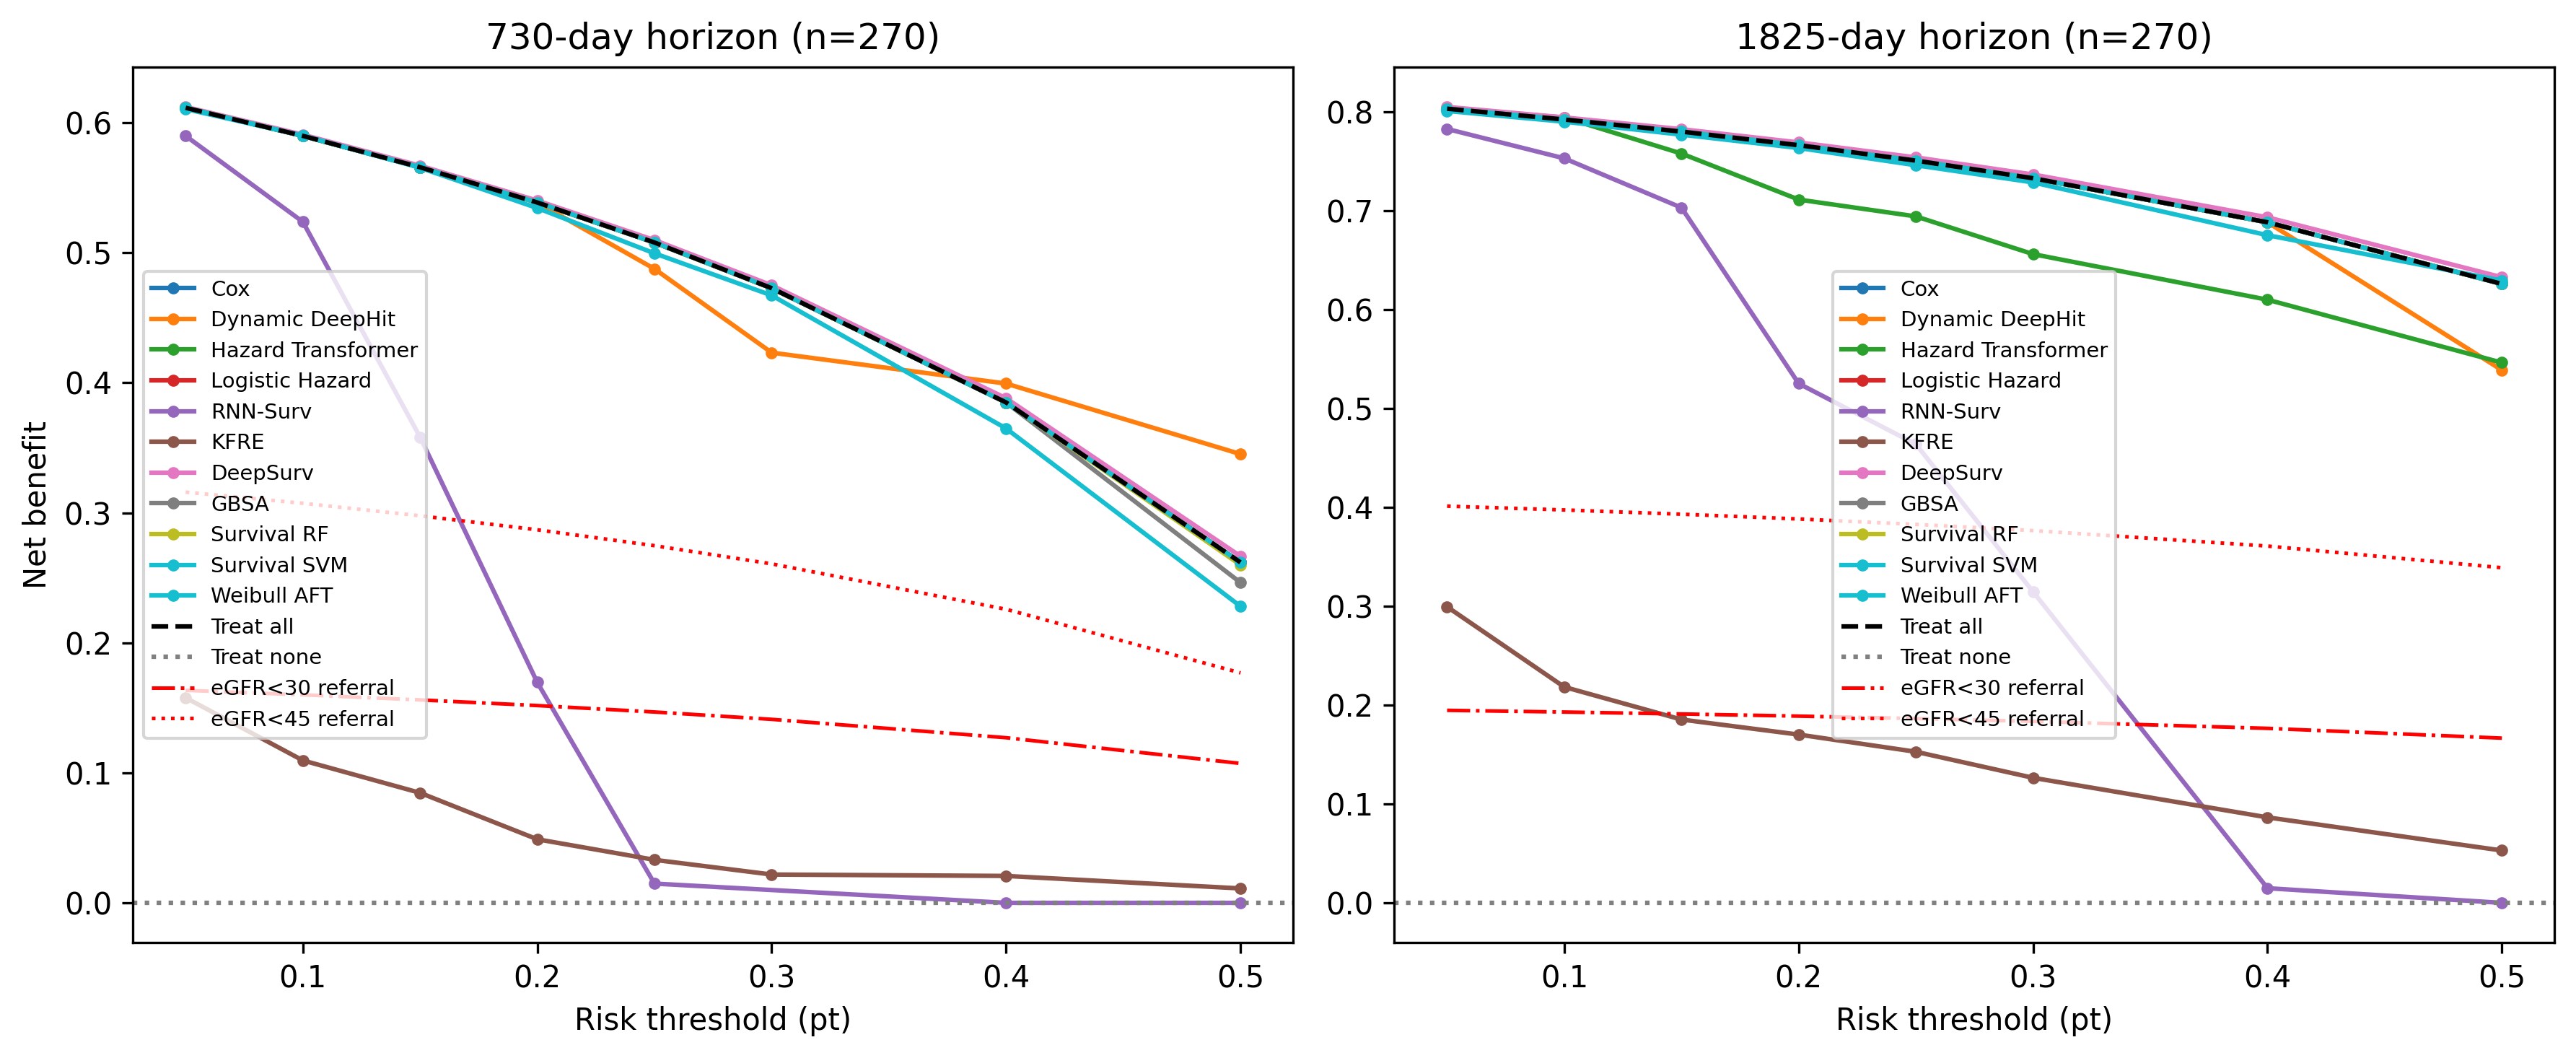
\includegraphics[width=\linewidth]{figs/four_features_decision_curve_plot.png}
    \caption{{\bf Four-feature holdout decision curves at 2 and 5 years (repetition 1).} Net benefit across risk thresholds for each model, treat-all, treat-none, and eGFR $<$30 and $<$45 referral rules, all evaluated on the same holdout patients and patient-level outcomes.}
    \label{fig:dca_four}
\end{figure*}


\end{document}
